
% sciences/science/assets/plot.tex

\begin{subfigure}{0.32\textwidth}\centering
	\begin{tikzpicture}
		\begin{axis}[width=1.2\linewidth, legend style={font=\tiny, at={(0.5, 1.05)}, anchor=south}]
			\addplot[variable=t]{t^4 + 3*t^3 - 12*t^2 + t - 6  };
			\addlegendentry{$f(t) = t^4 + 3t^3 - 12t^2 + t - 6$}
		\end{axis}
	\end{tikzpicture}
	\caption{Plot of $f(t)$}
\end{subfigure}
\hfill
\begin{subfigure}{0.32\textwidth}\centering
	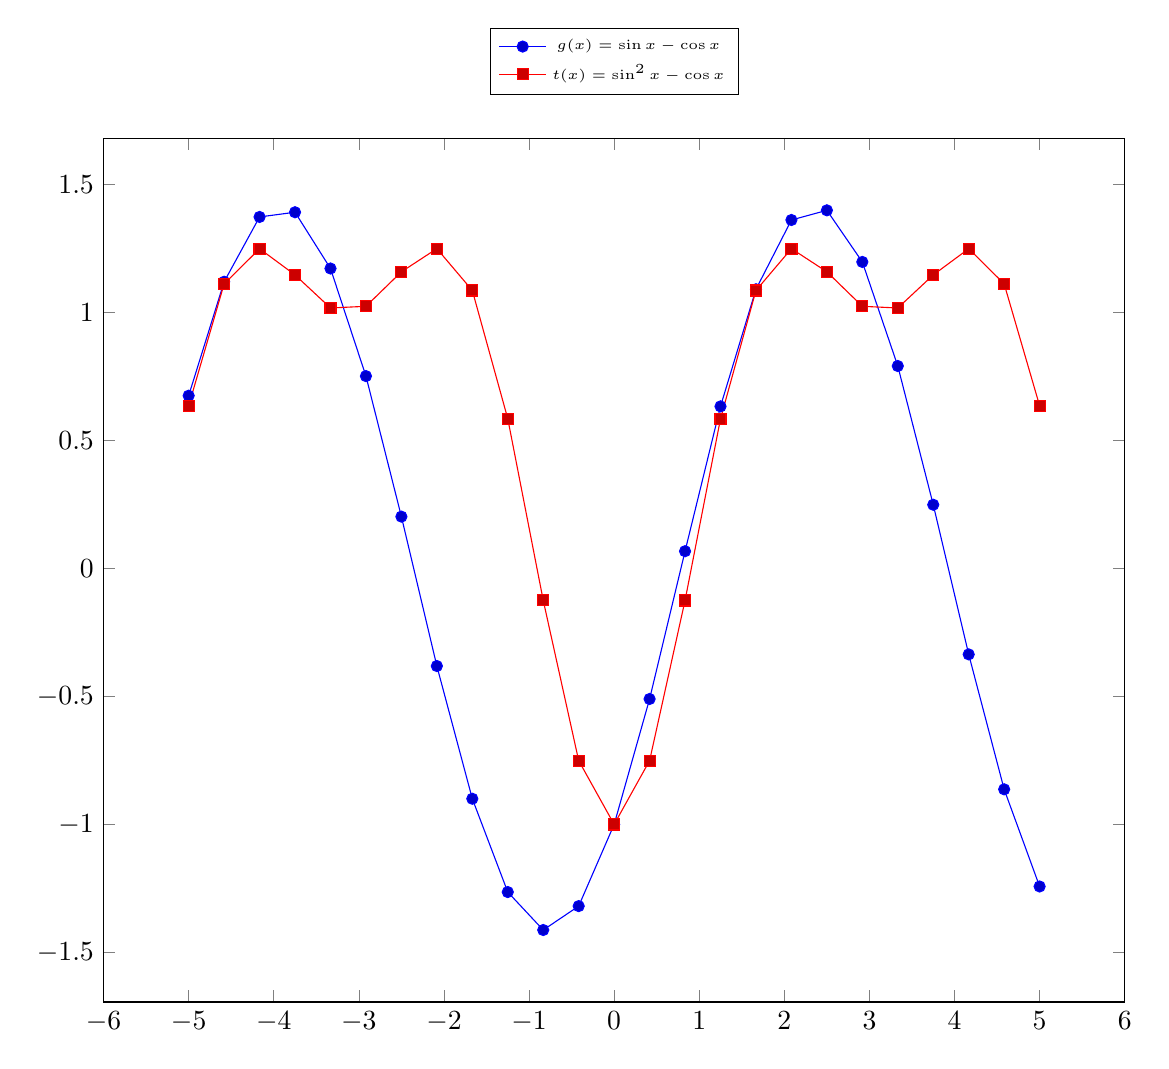
\begin{tikzpicture}
		\begin{axis}[trig format=rad, width=1.2\linewidth, legend style={font=\tiny, at={(0.5, 1.05)}, anchor=south}]
			\addplot{sin(x) - cos(x)};
			\addlegendentry{$g(x) = \sin x - \cos x$}
			\addplot{sin(x)^2 - cos(x)};
			\addlegendentry{$t(x) = \sin^2 x - \cos x$}
		\end{axis}
	\end{tikzpicture}
	\caption{Plot of $g(x)$ and $t(x)$}
\end{subfigure}
\hfill
\begin{subfigure}{0.32\textwidth}\centering
	\begin{tikzpicture}
		\begin{axis}[width=1.2\linewidth, legend style={font=\tiny, at={(0.5, 1.05)}, anchor=south}]
			\addplot[variable=\alpha]{e^(\alpha) + \alpha * ln(\alpha)};
			\addlegendentry{$\theta(\alpha) = e^\alpha + \alpha \ln \alpha$}
		\end{axis}
	\end{tikzpicture}
	\caption{Plot of $\theta(\alpha)$}
\end{subfigure}

